% Source ownership:
% - Itxaso: Serial Driver and Scientific Output
% - Itxaso: Python Post-Processing and Analysis
% - Oliwier: cleaned serial-results narrative and figure placement

\section{Serial Driver, Results and Post-Processing}
\label{sec:serial_post}

\subsection{Two-Phase Simulation Structure}

The updated serial workflow is built around a two-phase execution model:
an adaptive equilibration stage followed by a fixed-length production
stage. This is implemented in \texttt{main\_serial\_equil.f90}, where the
program first reads \texttt{input.dat}, constructs the initial polymer
geometry, and then decides whether equilibration should be performed
from scratch or bypassed through a previously saved equilibrated
configuration.

During Phase 1, the simulation performs Monte Carlo trial moves until
the Geweke convergence diagnostic declares that the energy time series
has reached a stationary regime. This replaces the old practice of
assigning an arbitrary burn-in length in advance. Once equilibration is
detected, the corresponding geometry is written to disk and becomes the
starting point for Phase 2.

Phase 2 is the production run proper. Here, the serial driver resets the
step counter and performs the requested number of Monte Carlo steps
starting from the equilibrated geometry. In the serial reference case
used throughout the report, this corresponds to a \(10{,}000{,}000\)-step
production simulation for a 500-carbon polyethylene chain with explicit
hydrogens at 300 K.

The driver records its scientific output periodically through the
\texttt{print\_interval} mechanism. At each output checkpoint, the code
writes the total, Lennard-Jones, and torsional energies together with
the main structural observables, especially the radius of gyration
\(R_g\) and the end-to-end distance \(R_{ee}\). Torsion-angle data and
trajectory snapshots are also written so that the structural evolution
can be visualised afterwards.

An annealing schedule is still retained in the serial code in the form
of a generic \(T_{\mathrm{ini}}\rightarrow T_{\mathrm{fin}}\) update.
For the simulations discussed here, however, the temperature is held
fixed at 300 K, so this block acts mainly as a configurable extension
point rather than a physically active part of the production protocol.

As a performance reference, the serial code was run on a single core of
an Intel Core i7-11800H processor. In the benchmark comparison used in
the report, one full serial production run required 8 hours, 18
minutes, and 31.91 seconds. This timing serves as the baseline against
which the parallel implementations were later compared.

\subsection{Automated Equilibration Detection}

The serial results are post-processed through \texttt{plot\_results.py}.
This script begins by parsing \texttt{input.dat} so it can detect
whether the run used explicit hydrogens and therefore decide which
theoretical torsional potential should be overlaid in the final
histogram plots. It then reads the separate equilibration and production
outputs and stitches them together into a single coherent visual
timeline.

For the energy and observable plots, the script concatenates the two
phases and marks the transition with a vertical dashed line. This makes
the time-demarcation between equilibration and production explicit and
allows the reader to assess whether the dynamics truly become stationary
after the detected equilibration point. By contrast, the torsional
distribution is generated using only the production portion, since that
is the only phase intended to represent equilibrium sampling.

The plotting layer is organized around three main functions:
\texttt{plot\_energies}, \texttt{plot\_observables}, and
\texttt{plot\_torsions}. The first plots the total, Lennard-Jones, and
torsional energies as functions of Monte Carlo step. The second plots
\(R_g\) and \(R_{ee}\). The third constructs the torsional histogram and
superposes the corresponding theoretical torsional potential using the
appropriate coefficient set for either the TraPPE-UA or OPLS-AA
effective model.

Before the runtime Geweke detector was introduced, a post-processing
equilibration analysis was also used as a diagnostic layer. In that
approach, the Python workflow estimated the integrated autocorrelation
time \(\tau_{\mathrm{int}}\) from the energy series by computing the
autocorrelation function through an FFT-based convolution. This
provides a fast way to estimate correlation lengths and effective sample
sizes even for long trajectories.

That legacy Python analysis remains useful as a cross-check because it
gives a purely post hoc view of correlation decay, burn-in length, and
statistical inefficiency. However, it was not always robust enough to
control the simulation by itself. In practice, long correlated plateaus
could distort the variance estimates and lead to pathological
truncations, including cases where the inferred production segment
became unreasonably short. This limitation was one of the main reasons
for moving equilibration detection into the Fortran runtime loop via the
Geweke criterion.

The final post-processing pipeline therefore combines two roles. The
Fortran code performs the actual online equilibration detection and
separates the simulation cleanly into equilibration and production, and
the Python code acts as the analysis and visualization layer that
verifies, displays, and interprets the resulting time series and
distributions.

\subsection{Serial Version Simulation Results}

The serial reference simulation consists of a Geweke-terminated
equilibration run followed by a $10{,}000{,}000$-step production run
for a 500-carbon polyethylene chain with explicit hydrogens at 300\,K.
The chain starts from a highly extended configuration generated by
\texttt{conf\_type\,=\,4}.

\begin{figure}[htbp]
  \centering
  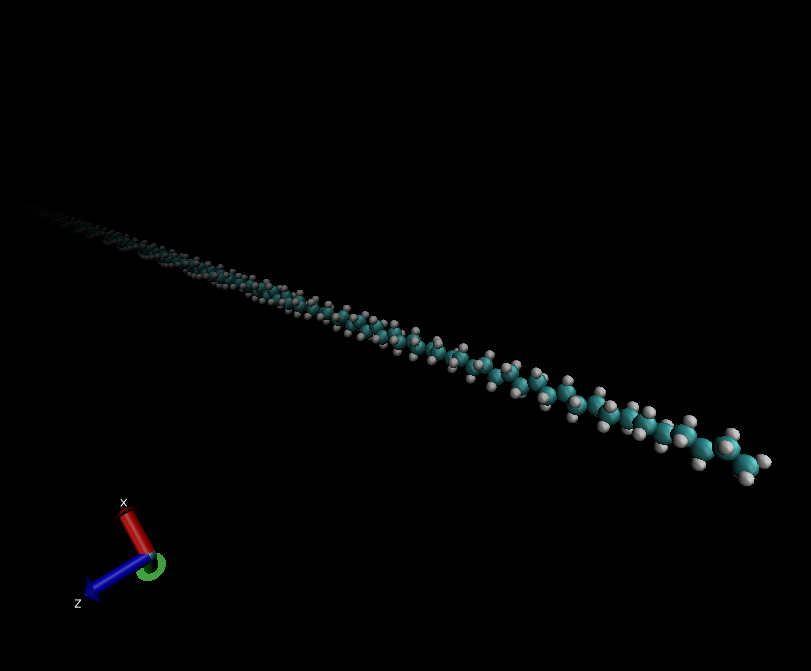
\includegraphics[width=0.48\textwidth]{figs/serial_geweke/VMD_serial_geweke_initial_geometry.png}
  \hfill
  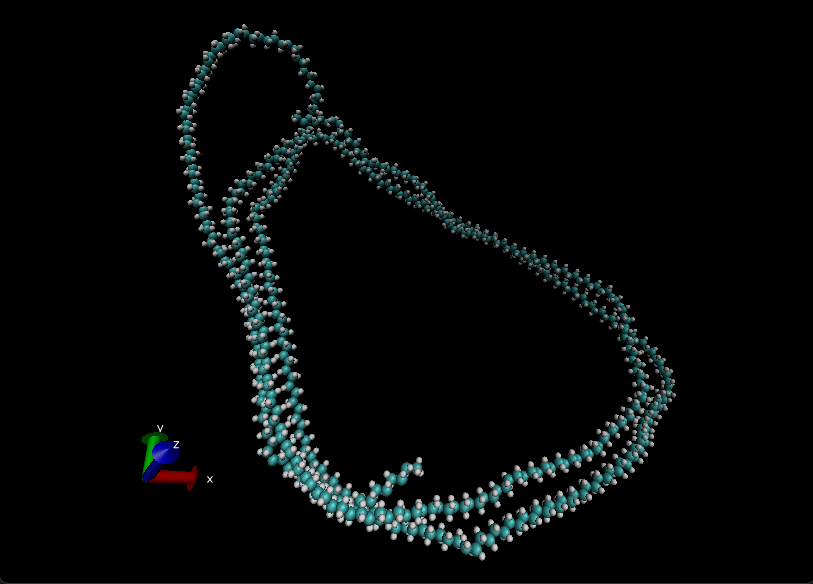
\includegraphics[width=0.48\textwidth]{figs/serial_geweke/VMD_serial_geweke_final_geometry.png}
  \caption{Left: initial configuration -- a nearly fully extended chain
    with all backbone carbons approximately collinear.
    Right: final production configuration -- a large open loop, 
    characteristic of a random-coil state.}
  \label{fig:vmd}
\end{figure}

The two VMD snapshots in Figure~\ref{fig:vmd} illustrate the scale of
the conformational change. The initial chain is nearly straight,
occupying roughly 650\,\AA\ end to end. The final structure is a
large folded loop with the two chain termini close together, far more
compact but not a dense collapsed globule.

\subsubsection{Structural Observables}

\begin{figure}[htbp]
  \centering
  
\includegraphics[width=0.8\textwidth]{figs/serial_geweke/observables_evolution_500_4_10000000_300.00.pdf}
  \caption{Radius of gyration $R_g$ (top) and end-to-end distance $R_{ee}$
    (bottom) across equilibration and production. The dashed vertical
    line marks the Geweke equilibration boundary at ${\approx}3.9 \times
    10^6$ steps.}
  \label{fig:observables}
\end{figure}

Figure~\ref{fig:observables} shows $R_g$ and $R_{ee}$ plotted
continuously across equilibration and production. $R_g$ begins at
approximately 185\,\AA\ and collapses to ${\approx}39$\,\AA\ within
the first 300\,000 steps, after which it fluctuates by only ${\sim}1$\,\AA\
around its mean for the remainder of the run. $R_{ee}$ follows a similar
rapid collapse from ${\approx}650$\,\AA\ to ${\approx}75$\,\AA, but
shows larger fluctuations in production (${\sim}15$\,\AA\ peak-to-peak),
which is expected: unlike $R_g$, which averages over all atoms, $R_{ee}$
depends only on the two terminal carbons and is therefore more sensitive
to large-scale rearrangements of the chain ends.

Both observables had converged well before the Geweke criterion declared
equilibrium at ${\approx}3.9 \times 10^6$ steps.

\subsubsection{Energy Evolution}

\begin{figure}[htbp]
  \centering
  
\includegraphics[width=0.8\textwidth]{figs/serial_geweke/energy_evolution_500_4_10000000_300.00.pdf}
  \caption{Total, Lennard-Jones, and torsional energy across
    equilibration and production. Dashed line marks the
    equilibration boundary.}
  \label{fig:energy}
\end{figure}

Figure~\ref{fig:energy} shows the three energy components. At step 1, the total energy is approximately 200\,kcal/mol, with the LJ term slightly negative around ---25\,kcal/mol (the extended chain has few close non-bonded contacts) and the torsional term near 230\,kcal/mol. Within the first million steps the chain folds rapidly, driving the LJ energy from ${\approx}{-25}$ to ${\approx}{-150}$\,kcal/mol as many atom pairs enter the attractive region of the LJ well simultaneously. The total energy settles to ${\approx}50$\,kcal/mol ($= {-150} + 200$\,kcal/mol from the two components). The torsional energy changes comparatively little (230 to 200\,kcal/mol), indicating that local torsional relaxation is much faster than global chain reorganization and that the initial configuration already had a broadly reasonable dihedral distribution.

After the equilibration boundary all three quantities fluctuate
stably, with no systematic drift visible over the full 10 million
production steps.

\subsubsection{Torsion Angle Distribution}

\begin{figure}[htbp]
  \centering
  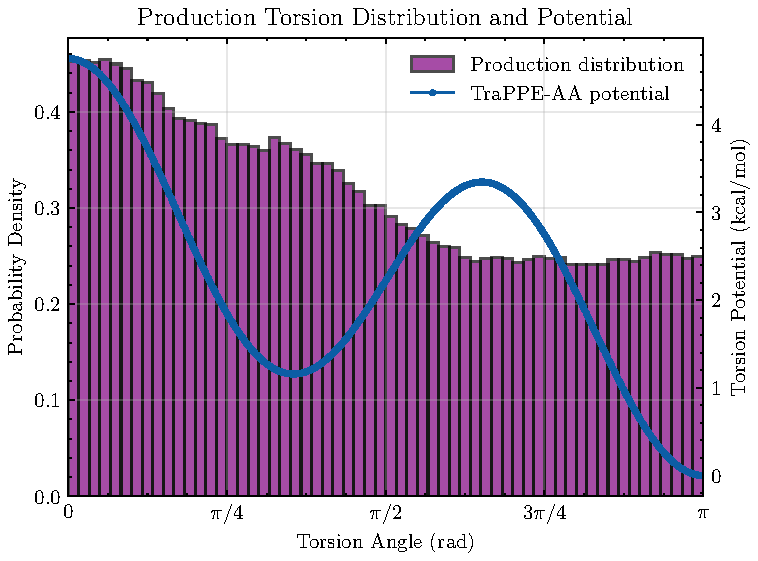
\includegraphics[width=0.8\textwidth]{figs/serial_geweke/torsion_distribution_500_4_10000000_300.00.pdf}
  \caption{Production-phase torsion angle distribution (purple
    histogram) overlaid with the OPLS-AA effective backbone potential
    (blue curve, right axis).}
  \label{fig:torsion}
\end{figure}

Figure~\ref{fig:torsion} shows the production torsion angle
distribution alongside the OPLS-AA effective backbone potential.
The histogram is concentrated almost entirely near $\phi = \pi$,
with the rest of the angular range essentially unoccupied. A small
gauche shoulder is visible near $\phi \approx \pi/3$, and the cis
region ($\phi \approx 0$) is absent from the distribution. This
population hierarchy is consistent with the potential: the global
minimum is at $\phi = \pi$ ($U = 0$), the gauche well sits
approximately 1.2\,kcal/mol above it, and the cis barrier reaches
approximately 4.7\,kcal/mol -- large relative to
$k_BT = 0.59$\,kcal/mol at 300\,K.

The equilibrium torsional energy of approximately 200\,kcal/mol
visible in Figure~\ref{fig:energy} is consistent with this
distribution. The torsional potential rises steeply from its
minimum at $\phi = \pi$, so small thermal fluctuations within
the trans well already carry a non-zero energy contribution per
dihedral. Summed across all backbone dihedrals, these
fluctuations account for the observed $E_{\mathrm{tors}}$ without
requiring significant population outside the trans region.

\subsection{Interpretation}

The simulation results are consistent with expected polymer behaviour
at 300\,K. The chain collapses from its initial extended geometry
within a few hundred thousand steps, after which it samples a
stationary conformational ensemble -- a compact random coil with
$R_g \approx 39$\,\AA\ and $R_{ee} \approx 75$\,\AA. These values
are substantially smaller than the fully extended length
(${\approx}650$\,\AA) but much larger than a fully collapsed globule
would give ($R_g \lesssim 15$\,\AA), confirming that the chain is in
a random-coil rather than a globular state.

The dominant contribution to energy stabilisation upon folding is
the Lennard-Jones term. In the extended configuration, most atom pairs
are beyond the LJ cutoff. As the chain folds, a large number of
non-bonded contacts accumulate in the attractive $r^{-6}$ region,
releasing ${\approx}125$\,kcal/mol of LJ energy. This is the
thermodynamic driving force for collapse at 300\,K.

The torsional distribution is governed by the total energy, not the
torsional term in isolation:
\begin{equation}
  E_{\mathrm{tot}} = E_{\mathrm{LJ}} + E_{\mathrm{tors}}.
\end{equation}
The Metropolis criterion accepts or rejects moves based on $\Delta E_{\mathrm{tot}}$.
Despite this coupling, the resulting torsional distribution is
dominated by the trans state in agreement with the
torsional potential hierarchy, because the torsional barriers are
large relative to $k_BT = 0.59$\,kcal/mol at 300\,K.
